\chapter{Considerations}\label{considerations}

\section{Architectural designs in question}
As the requirements have been set, we can examine the different ways the generation of the model could be
moved to a separate server. In this section, I'll go into detail about the different architectures that came up during
the planning phase. Last, but not least, I'll explain, why I chose the WebSocket implementation after carefully researching
my possiblilites.

\subsection{REST API}\label{restconsiderations}
The first architecture that came to my mind, was a \textbf{REST API (subsection \ref{backgrrestapi})}. Using the Spring boot framework would allow for fast development
of our REST API. The state of the partial modelling editor would be sent to the REST API as a POST request, and the result
would be returned as a Json, which the client would parse, and output the model accordingly. However, it was still in question
how the generated model should be returned to the client.
\begin{itemize}
        \item \textbf{Long return:}
		The first implementation that came up, was a regular REST API, where the response of the API would only be received, after
		the model generation had been finished. An implementation plan can be seen in figure \ref{longreturnimage}. 
		As we know REST responses shouldn't take a long time to respond to received requests.
		The Generator is probably the slowest service of Refinery, so responding with the model details may take a fairly long time.
		As such, the purpose of a single request - single response REST API would be invalid / way too slow for our usecase.
		\begin{figure}
			\begin{center}
				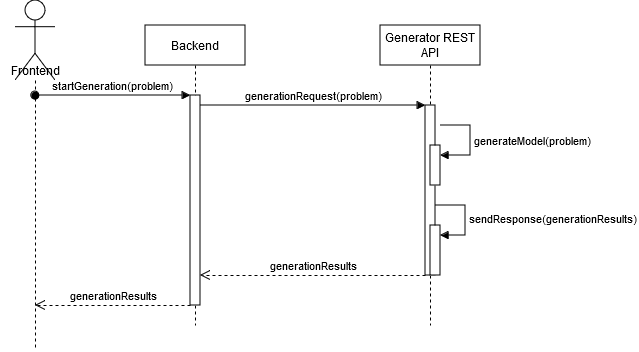
\includegraphics[scale=0.6]{include/imgs/rest_long_return.png}
				\caption{Possible long return implementation of generator REST API}
				\label{longreturnimage}
			\end{center}
		\end{figure}
		\item \textbf{Long polling:}
		Here, the REST API would respond immediately with a "Starting generator service" message, had it received a request.
		The REST API would start and perform the generation, while the backend would constantly try to fetch the results from the API.
		An example implementation can be seen in figure \ref{longpollingimage}
		\begin{figure}
			\begin{center}
				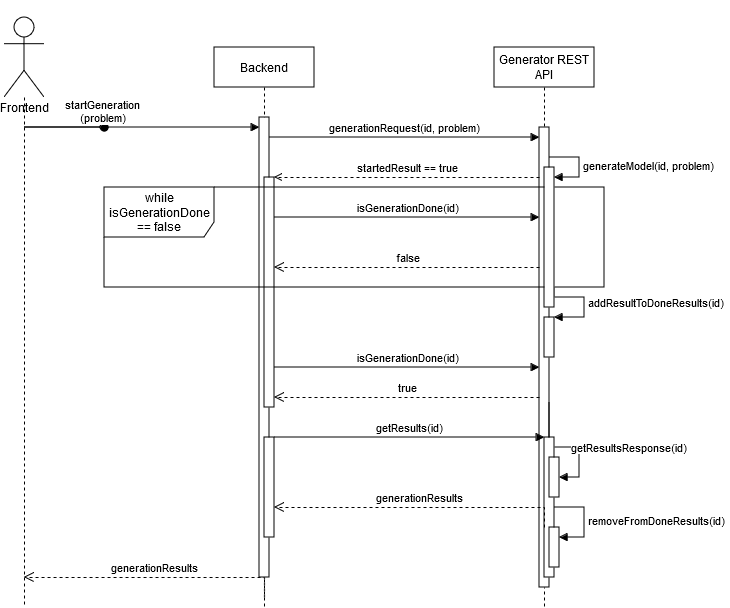
\includegraphics[scale=0.5]{include/imgs/rest_long_poll.png}
				\caption{Possible long polling implementation of generator REST API}
				\label{longpollingimage}
			\end{center}
		\end{figure}
\end{itemize}
The limitation of both implementations is the fact that the request cannot be cancelled from the client side. As that is one 
of the main requirements of the architectural restructuring, this is a fact that cannot be looked over, so I concluded that 
another architecture should be looked at for the implementation.


\subsection{Remote Procedure Call} \label{rpcconsiderations}
	The second architecture that came up during the planning phase was Remote Procedure Call (RPC) (section \ref{backgrpc}). The generation is pretty much
	a procedure, so calling it remotely sounded like a wise choice. 

	Using gRPC (section \ref{backgrgrpc}) would provide the timeout logic, and other clients
	could also be created in the future, as the generator server would function as a gRPC server. The newly created clients would only need to
	act as a gRPC client, and send requests according to the server's specification.

	gRPC would allow us to use a one request - multiple responses implementation, for representing the current state of the generation.
	The cancellation of the generation can also be done via gRPC's provided cancelation code examples. The thread running the generation of
	the model could be stopped upon receiving a cancel request.

	gRPC communicates over HTTP 2.0, so the newer HTTP protocol would have to be used, in order to utilize the usage of the gRPC library.

\subsection{WebSocket server} \label{considerationwebsocket}
	Last but not least, comes WebSocket (section \ref{backgrwebsocket}). This basically would work the same way as the REST API long polling implementation,
	however, the connection would not be closed after the initial request. This is due to the way WebSocket works.
	
	Due to the nature of WebSocket, after the model generation request is sent out by the client,
	the connection is kept alive, and the server may send back multiple responses over the same connection.
	This comes in handy for the representation of the state. The server can continously send to the client,
	where the model generation is currently at.

	The current implementation for the communication between the web client and the editor server is already using a WebSocket connection.
	As such, the same cancelation and timeout logic can be applied for the generator server, meaning that those two requirements would also be satisfied.
	After all of these considerations WebSocket seemed like the best implementation moving forward, but the way it would be implemented
	had still to be decided:

	\begin{itemize}
			\item \textbf{Using a separate connections from the webclient side}
			This way, the webclient (or "frontend") would be the one making a connection with the generator server. This way
			there would be two connections created from the webclient: one towards the generator server, and a separate one 
			towards the editor server.

			\item \textbf{Using the same connection as the editor}
			In this implementation, the editor server (backend) would function as a "proxy" towards the generator microservice. This is made possible 
			by the fact that in the current implementation, the webclient already makes a WebSocket connection towards the editor server, and 
			the editor server is the one performing the generation.
	\end{itemize}

\subsection{Decision} \label{archdecision}
	After investigating and evaluating the possible implementations, I decided to choose the WebSocket implementaiton 
	utilizing the `backend as a proxy towards the microservice' due to the reasons below.

	The \textbf{REST API implementation} should not be used as the states where an ongoing generation stands (see section \ref{requirements} 
	requirement number \ref{requirementstate}) would be hard to represent
	without the use of a workaround. Furthermore, the cancelation of ongoing generations (see section \ref{requirements} 
	requirement number \ref{requirementcancel}) would also need some workarounds for it to be implemented.

	The \textbf{gRPC implementaiton} could satisfy all of the project requirements. The The ongoing generations could be cancelled (see section \ref{requirements} 
	requirement number \ref{requirementcancel}) and timeouts could 
	be handled too (see section \ref{requirements} 
	requirement number \ref{requirementtimeout}). 
	The gRPC implementation would introduce new dependencies for both the backend and the generator server projects.
	The final image of the backend and the generator would grow even bigger, but neither the overall user experience, performance
	or the scalability would be improved compared to the WebSocket implementation. 

	\begin{figure}[h!]
		\begin{center}
			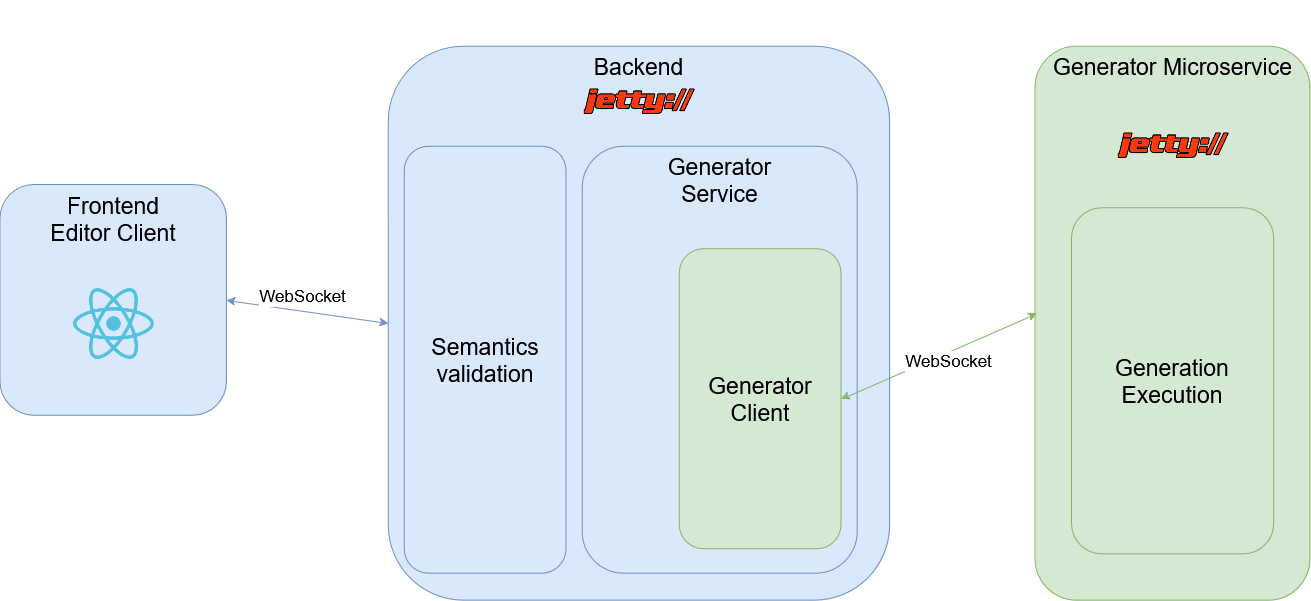
\includegraphics[scale=0.3]{include/imgs/arch_plan.png}
			\caption{Final proposed architectural changes}
			\label{archplan}
		\end{center}
	\end{figure}

	The \textbf{WebSocket implementation} proposed in figure \ref{archplan} could satisfy all of the project requirements (section \ref{requirements}). 
	Furthermore, WebSockets are already used 
	in the backend project so it should be straightforward to use in the microservice implementation aswell.
	This info also assures me, that there won't be any dependency issues related to this implementation. Another key factor, is that via the use of 
	WebSockets, no additional dependencies have to be added. The editor server already communicates with the clients over WebSocket, through which
	the model generation requests are sent over. Using WebSockets and the "backend as a proxy towards the microservice" (section \ref{considerationwebsocket}) implementation could 
	reduce the overall work needed for the refactor, 
	as the Frontend of Refinery 
	doesn't have to be touched. The changes to the architecture of the application will not be noticable for the client, yet the performance may improve.

\section{Infrastructure}

	Now that we have gone over the architectural changes that need to be implemented, we need to take a look at how the 
	scalability of the application is really going to be improved, and how the application should be deployed.
	For this I'll utilize Amazon Web Services, as it is one of the leading industry standard cloud providers
	and the current Refinery is also deployed on AWS platforms.

	AWS currently offers many options for running our application, both server and serverless methods.
	When thinking about server methods, the ways include EC2, ECS, EKS. When talking about serverless approaches
	Fargate and Lambda are the solutions that come to mind. In the following section I'll describe how each of these
	services could be used for our infrastructure, and come to a conclusion, of how our infrastructure will be deployed.
	When deciding about the infrastructure, the key considerations are going to include the specifications for our microservice,
	how easy it is to maintain our deployed application, and last, but not least the costs affiliated with said infrastructure.


	\subsection{Elastic Compute Cloud (EC2)}
		Amazon EC2 is basically a fully functional VM instance on Amazon's infrastructure. This is the most bare-bones approach as this
		would be the same, as running a linux server on any on-prem instances. 
		By containerizing our application, no additional libraries
		would need to be installed: we just need to run our docker image, and the container would be ready to go. 
		
		Another advantage of this approach
		is the price. This is one of the cheapest services of Amazon, with instance hourly rates starting as little as \$0.0048, to going as high as 
		\$0.1728 for a single instance (key factors in pricing include CPU cores, memory and network performance).

		However, advantages of this approach stop right there. When it comes to maintaining our application, EC2 doesn't offer much.
		On the AWS dashboard, we could see, whether our instance is running, but nothing about the state of our application running in 
		the docker container. Another disadvantage, is that scaling is pretty much non-existent from the get-go. Auto Scaling Groups and Load Balancers
		can be created by using EC2 instances, but the setup of them is tedious. 

	\subsection{Serverless approaches (Fargate and Lambda)}
		As our generator application is gonna be containerized, serverless options such as AWS Fargate and AWS Lambda can come into play.
		
		With AWS Fargate, one of the main advantages is that only real computing usage is billed, and
		downtimes aren't billed, when the service isn't used. 

		However, in practice, prices associated with Fargate seem to be 
		much higher, compared to EC2 instance hourly rates: \$0.04656 dollars per CPU core and \$0.00511 per GB per hour. As a
		result, Fargate sounds great on paper, but with increased usage monthly costs can increase significantly.

		With AWS lambda, there would not be a need for containerization, as AWS runs code snippets from compressed ZIP folders, if the code 
		snippets are in supported languages. AWS lambda supports java, so that is a possibilty. The pricing depends on the memory that 
		we allocate for our lambda functions and the amount of time they take to complete. If we were to allocate 512MB of memory for 
		our function, the price per 1ms in the Europe region would be \$0.0000000083. That price sounds better than the former two options. 
		However, lambda is usually used for non-resource demanding codes. As such, the response times could become much worse than if we 
		were to run the generation with a Fargate or EC2 approach.

		Both solutions would allow for scaling. Fargate scales horizontally meaning that the number of instances running can be increased.
		Lambda scales vertically, with the resources allocated for the function. 

		Most crucially, the biggest downside of running our microservice with a serverless approach is that it would not satisfy many requirements
		that were made in the application specification. If a generation would be cancelled by the user, there would be no easy way of cancelling it, 
		as essentially these services are running code snippets, where runtime modification is not possible without workarounds / AWS SDK usage. This 
		would also make our application dependent on AWS, as the migration to a different cloud provider / deployment on a local instance would get more
		complicated, or even impossible, without changes to the codebase. 

		Last, but not least, the state of the generation would be tedious to send back to the backend and the frontend. 
		We would either have to give up on the
		generation state representation, or create some kind of workaround (such as an API endpoint) where the state of the generation is
		stored. However, that would make the infrastructure much more complicated, and the whole premise of a serverless approach would 
		be destroyed.

		After all of these considerations, I have decided to give up on a serverless approach, as the drawbacks of such implementation
		outweight the advantages of reduced costs, that could happen with low application usage.
		

	\subsection{Elastic Container Services (ECS)}
		Amazon ECS allows for setting up container tasks and running them inside services. Tasks can be run using EC2 or AWS Fargate instances.
		The amount of vCPUs and memory allocated for each container can also be configured.
		Setting up an ECS cluster has no additional costs affiliated with it, other than the cost of the running EC2 or Fargate instances.

		Scaling can be made possible via the usage of auto scaling groups and load balancers. Within auto scaling groups, we can define how many
		running instances we want to allow our services to scale up to. The triggering effects can also be set, such as average CPU utilization and 
		average memory usage. If our task reaches that treshhold, a new instance of the task is launched.  
		The load balancers immediately register the running instances within the auto
		scaling group, so that would also make the implementation pretty straightforward. The load balancer can forward traffic to generator 
		microservice instances based on their routing algorithm, which can either be set as a round-robin or least connections.

		ECS also helps the maintanence of the infrastructure. AWS can collect many logs associated with 
		the container tasks. Monitoring of the resource usages can also be done via AWS management console dashboards.

		Due to the drawbacks of a serverless implementation listed in Serverless approaches, it would be beneficial to use EC2 instances
		for the running of our containers. That implicates that the implementation has to be done in a way, where our docker container (generator
		microservice) acts as a server.

	\subsection{Kubernetes}
		Kubernetes could be used as a tool for container orchestration, without the need of any provisioning tools. 
		However, the project is mainly related to the creation of a generator
		microservice and removing the generation from the main backend. As a result, I feel like using 
		Kubernetes or Elastic Kubernetes Service (EKS) for this task
		would be way too overkill, as only two containers would be running at the same time. 
		For a task of this size, the YAGNI principle (= `You are not gonna need it') should be applied.
		
		EKS wouldn't even allow us to become more independent
		from the AWS infrastructure (as if that was an issue, with only docker containers being hosted as tasks). However, if using another 
		public cloud provider was be an aspect, that we would need to consider, this would be a viable option. Kubernetes also allows for 
		greater customizability of auto scaling properties.

	\subsection{Decision} \label{awsdecision}
		The final deployment of our infrastructure will be done via the use of ECS and EC2 instances running the defined container tasks.
		The tasks should be running on the same auto scaling group of EC2 instances. 
		
		A load balancer will be added, so that the 
		network traffic can be forwarded to the tasks running our docker containers. The cost of an application load balancer is \$0.02394 per Application 
		Load Balancer-hour in the Stockholm region, where I am planning to deploy the application in the future. This application load balancer
		will balance the traffic towards basic backend target groups, and also towards generator server instances.

		Another key factor, is that Amazon has cheaper prices for EC2 instances with arm cpu architecture. It would be beneficial
		to create a multi-architectural docker images, so that when we deploy our application, cheaper running costs can be 
		achieved.

		With this plan, using t3a.micro arm EC2 instances, the costs associated with the deployment should be as follows:
		
		\begin{center}
			Minimum cost per hour = $2 \times \$0.0108$ + \$0.02394 = \$0.04554
		\end{center}

		So approximately 4.6 cents per hour. This includes the usage of two EC2 instances and an Application Load Balancer.

		\begin{figure}[h!]
			\begin{center}
				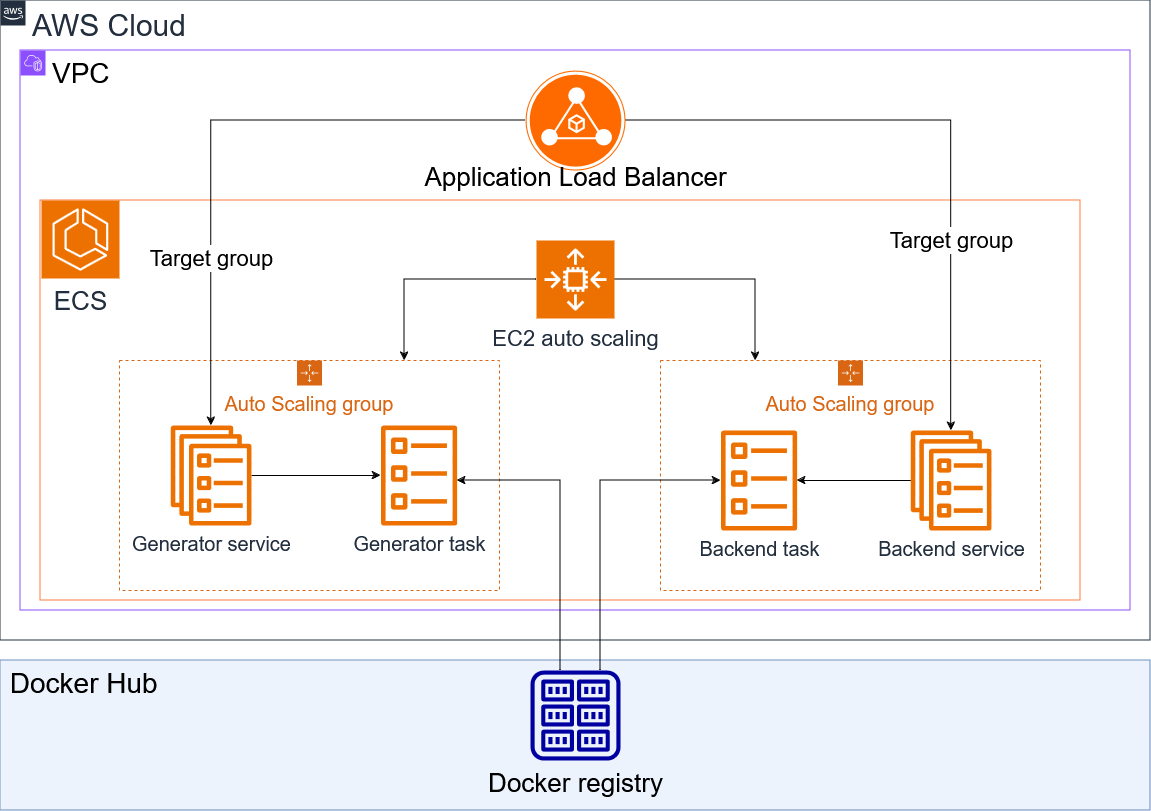
\includegraphics[scale=0.35]{include/imgs/aws_infra_plan.png}
				\caption{Final proposed infrastructure for deployment}
				\label{infraplan}
			\end{center}
		\end{figure}